\documentclass{beamer}

\mode<presentation>
{
  \usetheme{Warsaw}
  \setbeamercovered{invisible}
}

\setbeamertemplate{navigation symbols}{}

\graphicspath{{./images/}}

\usepackage[english]{babel}
\usepackage{times}
\usepackage[latin1]{inputenc}
\usepackage[T1]{fontenc}
\usepackage{lmodern}
\usepackage{amsmath,amsthm,amssymb}
\usepackage{hyperref}
\usepackage{nccfoots}
\usepackage{subfigure}
\usepackage{outlines}

\renewcommand\thempfootnote{*}

\renewcommand{\t}{$\mathrm{t}$ }
\newcommand{\BHV}{$\mathrm{BHV}$ }
\newcommand{\NP}{$\mathrm{NP}$ }
\newcommand{\MCMC}{$\mathrm{MCMC}$ }
\newcommand{\SPR}{$\mathrm{SPR}$ }

\newcommand{\dts}{\mathrm{2DtT}}
\newcommand{\nni}{\mathrm{NNI}}
\newcommand{\rnni}{\mathrm{rNNI}}
\newcommand{\rnniu}{\mathrm{rNNIu}}
\newcommand{\mdts}{\mathrm{DtT}}
\newcommand{\mdtsu}{\mathrm{DtTu}}
\newcommand{\MH}{\mathrm{MH}}
\newcommand{\ric}{\operatorname{ric}}
\newcommand{\rt}{\mathrm{rt}}
\newcommand{\tp}{\mathrm{tp}}
\newcommand{\W}{\mathcal{W}}
\newcommand{\M}{\mathcal{M}}
\newcommand{\dom}{\mathrm{dom}}

\renewcommand{\O}{\mathcal{O}}

\newtheorem{oobservation}{Trivial observation}

\theoremstyle{example}
\newtheorem{question}{Question}

\title[\url{https://gavruskin.github.io/talks/2016_Evolution.pdf}]{Next generation phylogenetic inference @Evolution2016:\\
Nearest neighbors of phylogenetic time-trees}
\author[These slides:]{Alex Gavryushkin\\
(joint work with Chris Whidden and Erick Matsen)}
\titlegraphic{\includegraphics[height=2cm]{UniAuckland}}

\date{June 20, 2016}


\begin{document}

\begin{frame}[plain]
\setbeamertemplate{footline}{}
\titlepage
\end{frame}


\addtocounter{framenumber}{-1}
\addtobeamertemplate{navigation symbols}{}{
	\usebeamerfont{footline}
	\usebeamercolor[fg]{footline}
	\hspace{1em}
	\insertframenumber/\inserttotalframenumber
}


\begin{frame}{Motivation}
\begin{block}

\begin{outline}
\1 General statistics is at least $5$ years ahead of phylostatistics.
\pause
\1 The discrete component of tree space is \emph{the} bottleneck for tree search algorithms.
\pause
\1 What's wrong with trees?
\end{outline}
\end{block}

\pause

\begin{block}{Same as above but with a mortarboard on}
\begin{outline}
\1 \MCMC algorithms
	\2 Improving efficiency $=$ smart proposals
	\2 Point estimates AKA posterior summary
\1 Tree search methods in general
	\2 Semi-convergence
	\2 Valleys
	\2 Terraces
\end{outline}
\end{block}
\end{frame}

\begin{frame}
THESE ARE NOT THE TYPE OF TREES WE'RE GONNA CONSIDER --- ?
\end{frame}

\begin{frame}
\begin{block}{(Discrete) Time-tree}
\includegraphics[width=\framewidth]{discreteTimeTree}
\end{block}
\end{frame}

\begin{frame}
\begin{block}{Discrete time-tree space}
\includegraphics[width=\framewidth]{DtT}
\end{block}
\end{frame}

\begin{frame}
\begin{block}{Trees at distance $3$}
\includegraphics[width=\framewidth]{dts_neighbors}
\end{block}
\end{frame}

\begin{frame}{Looks promising!}
\begin{block}{G, Whidden, and Matsen, arXiv, to appear in June 2016}
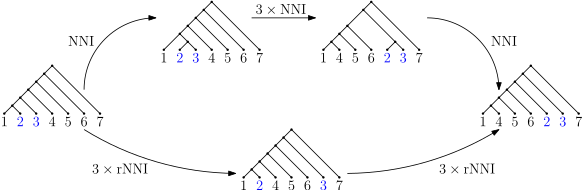
\includegraphics[width = \framewidth]{NNI_VS_rNNI}
\end{block}
\end{frame}

\begin{frame}{Promising indeed}
\begin{block}{G and Drummond, JTB 2016}
\includegraphics[width=\framewidth]{tauSpace}
\end{block}
\end{frame}

\begin{frame}{\href{http://alex.gavruskin.com/pictures/}{\Large{Thank
you for your attention!}}}
\thebibliography{9}
\bibliographystyle{alpha}

\scriptsize

\bibitem{Ollivier}
Yann Ollivier
\newblock Ricci curvature of Markov chains on metric spaces
\newblock {\em J.\ Functional Analysis,} 256, 3, 810--864, 2009

\bibitem{Gavruskin2015}
Alex Gavryushkin and Alexei Drummond
\newblock The space of ultrametric phylogenetic trees
\newblock {\em arXiv preprint} \href{http://arxiv.org/abs/1410.3544}{arXiv:1410.3544}, 2014

\bibitem{chrisErick}
Chris Whidden and Frederick A.\ Matsen IV
\newblock Quantifying MCMC exploration of phylogenetic tree space
\newblock {\em Systematic Biology}, doi:10.1093/sysbio/syv006, 2015

\bibitem{chrisErick2015}
Chris Whidden and Frederick A.\ Matsen IV
\newblock Ricci-Ollivier curvature of two random walks on rooted phylogenetic subtree-prune-regraft graph
\newblock To appear in the proceedings of the {\em Thirteenth Workshop on Analytic Algorithmics and Combinatorics,} 2015

\bibitem{chrisErickG2015}
Alex Gavryushkin, Chris Whidden, and Frederick A.\ Matsen IV
\newblock Random walks over discrete time-trees
\newblock To appear on the {\em arXiv,} 2015

\bibitem{GavryushkinGitHub}
\url{https://github.com/gavruskin/tauGeodesic}

\bibitem{GavryushkinGitHub2}
\url{https://github.com/gavruskin/tTauCurvature}
\end{frame}
\end{document}
